%%%%%%%%%%%%%%%%%%%%%%%%%%%%%%%%%%%%%%%%%%%%%%%%%%%%%%%%%%%%%%%%%%%%%%%%%%%%%%%%
\subsection{Συμπεράσματα κεφαλαίου}
\label{subsection:02_01_05:01}

Σε αυτό το κεφάλαιο αξιολογήσαμε την επίδοση των τελευταίας τεχνολογίας πακέτων
λογισμικού \texttt{ROS} που είναι ικανά να φέρουν εις πέρας το έργο της
αυτόνομους πλοήγησης στο πεδίο εφαρμογής \ref{scope}. Οι αλγόριθμοι αυτοί είναι
δύο ειδών: αλγόριθμοι χάραξης μονοπατιών ανάμεσα σε δύο στάσεις του χάρτη του
περιβάλλοντος στο οποίο κινείται μία κινητή βάση ρομπότ, και αλγόριθμοι ελέγχου
της κίνησης του ρομπότ στο περιβάλλον του. Ο συνδυασμός τους αποτελεί τον
πυρήνα της πλοήγησης μίας κινητής βάσης ρομπότ άνευ εξωτερικών χειροκίνητων
χειρισμών της.

Η αξιολόγηση είχε ως στόχους
\begin{itemize}
  \item το σχεδιασμό μίας ολοκληρωμένης, περιεκτικής, και επεκτάσιμης
        μεθοδολογίας αξιολόγησης μεθόδων αυτόνομους πλοήγησης κινητών βάσεων
        ρομπότ, και
  \item την εφαρμογή της για την αξιολόγηση της επίδοσης τρεχόντων υλοποιήσεών
        τους μέσω του μεσολογισμικού \texttt{ROS}
\end{itemize}

Προκειμένου να διακρίνουμε τα εύρωστα και εύχρηστα πακέτα λογισμικού από τα μη,
συστήσαμε μία μεθοδολογία προκαταρκτικής αξιολόγησής τους με βάσει ποιοτικά
κριτήρια που τίθενται από την εμπειρία ανάπτυξης και συντήρησης λογισμικού.
Στη συνέχεια σχεδιάσαμε μία μεθοδολογία αξιολόγησης με βάση ποσοτικές μετρικές,
οι οποίες αποτελούν αντικειμενικά κριτήρια της επίδοσης ενός ρομπότ στο έργο
της αυτόνομους πλοήγησης, και στις οποίες ένας μηχανικός ρομποτικής μπορεί να
θέσει επιπλέον ή λιγότερο βάρος αναλόγως των σκοπών της εφαρμογής των εν λόγω
πακέτων αυτόνομους πλοήγησης. Έπειτα εφαρμόσαμε τη μεθοδολογία ποσοτικής
αξιολόγησης σε εννιά συνδυασμούς πακέτων, πραγματοποιώντας χρήση τους για
αυτόνομη πλοήγηση σε δύο ετερογενή προσομοιωμένα περιβάλλοντα και σε ένα
πραγματικό. Τα περιβάλλοντα και οι διαδρομές πλοήγησης επιλέχθηκαν έτσι ώστε
να δοκιμάσουν τους υποκείμενους αλγορίθμους με μία σειρά κριτηρίων, και με
κλιμακωτή δυσκολία. Το αποτέλεσμα ήταν μία ιεράρχηση των συνδυασμών των πακέτων
λογισμικού, στην κορυφή της οποίας βρίσκεται ένας συνδυασμός ο οποίος φέρει
εις πέρας το έργο της αυτόνομους πλοήγησης με ελάχιστα σφάλματα πλοήγησης,
σε εύλογους χρόνους, και, συνολικά, άριστη επίδοση στο σύνολο των τριών
περιβαλλόντων δοκιμής.


%%%%%%%%%%%%%%%%%%%%%%%%%%%%%%%%%%%%%%%%%%%%%%%%%%%%%%%%%%%%%%%%%%%%%%%%%%%%%%%%
\subsection{Αιτίες περαιτέρω έρευνας}
\label{subsection:02_01_05:02}

Για το σκοπό της αυτόνομους πλοήγησης είναι απαραίτητη η γνώση ή η εκτίμηση της
τρέχουσας στάσης του ρομπότ: μόνο με βάση αυτήν είναι δυνατή η εύρεση ταχυτήτων
προς είσοδο στους κινητήρες των τροχών της κινητής βάσης έτσι ώστε να
ακολουθείται το σχεδιασθέν μονοπάτι. Στο πεδίο εφαρμογής \ref{scope} η γνώση
της στάσης δεν είναι δυνατή: μόνο η παρατήρησή της είναι δυνατή, μέσω των
αισθητήρων που φέρει το ρομπότ (παρατήρηση \ref{remark:01}). Για την παρατήρηση
της στάσης του ρομπότ κατά τη διενέργεια της πειραματικής διαδικασίας
χρησιμοποιήσαμε το φίλτρο σωματιδίων (ενότητα \ref{subsec:01_01_02_3}).

Αυτό που παρατηρήσαμε δια ζώσης και με γυμνό μάτι κατά τη διάρκεια της
πειραματικής διαδικασίας ήταν ότι η εκτίμηση της στάσης του ρομπότ δεν σύναδε
πάντοτε με την πραγματική του στάση: σε λίγες περιπτώσεις παρατηρήσαμε ότι η
εκτίμηση της θέσης ταλαντωνόταν απότομα ανάμεσα σε μερικές υποψήφιες
θέσεις---σε άλλες στιγμές παρατηρούσαμε ότι η εκτίμηση της στάσης του ρομπότ
είχε ορατό σφάλμα σε σχέση με την πραγματική του στάση. Το σχήμα
\ref{fig:02_01_05} δείχνει την εξέλιξη του μέσου όρου των σφαλμάτων κατάστασης
(του διανύσματος της στάσης) κατά τις δέκα διαδρομές του συνδυασμού του ελεγκτή
\texttt{teb\_local\_planner} με τον αλγόριθμο χάραξης μονοπατιών \texttt{navfn}
στο περιβάλλον CORRIDOR (αριστερά) και με τον \texttt{global\_planner} στο
περιβάλλον WILLOWGARAGE (δεξιά). Σε αυτά τα σχήματα παρατηρούμε τέσσερα
πράγματα για το σφάλμα κατάστασης:
(α) δεν έχει σταθερά μηδενική (ή αμελητέα) τιμή,
(β) δεν έχει σταθερή τιμή μέσα στο χώρο και κατά τη διάρκεια του χρόνου,
(γ) δεν έχει παρόμοιες καμπύλες εξέλιξης σε διαφορετικά περιβάλλοντα, και
(δ) δεν έχει το ίδιο άνω ή κάτω όριο σε διαφορετικά περιβάλλοντα.\footnote{Από
την ανάλυση των αποτελεσμάτων για όλους τους συνδυασμούς αλγορίθμων χάραξης
μονοπατιών με ελεγκτές κίνησης προκύπτει, όπως είναι εύλογο, ότι το σφάλμα
κατάστασης είναι ανεξάρτητο από αυτούς.}

Ανάλογα με τους σκοπούς ρομποτικών εφαρμογών το σφάλμα κατάστασης μπορεί να
έχει μεταβλητές προδιαγραφές. Για παράδειγμα, σε αποθήκες με μεγάλους χώρους και
πλατειά περάσματα, όπου ο στόχος είναι η απογραφή της θέσης προϊόντων με αδρή
ακρίβεια θέσης (της τάξης των δεκάδων εκατοστών του μέτρου), ούτε η πλοήγηση
δυσχεραίνεται, ούτε και διαταράσσεται η ακρίβεια της απογραφής. Αντιθέτως,
σε περιβάλλοντα με στενά περάσματα ή απαιτήσεις ακριβείας στάσης (για παράδειγμα
σε αυτόνομα παλετοφόρα οχήματα), η αυτόνομη πλοήγηση δυσχεραίνεται σε αναλογία
με το σφάλμα στάσης και το πόσο στενά είναι τα περάσματα, και το έργο που
απαιτεί ακρίβεια στάσης του ρομπότ (η φόρτωση των παλετών από το όχημα) σε
αναλογία με το μέγεθος του σφάλματος στάσης. Στο πλαίσιο της βιομηχανίας η
ελάττωση του σφάλματος εκτίμησης της στάσης ενός αυτόνομου ρομπότ προς το παρόν
επιτυγχάνεται είτε με επιπρόσθετο και κοστοβόρο εξοπλισμό, είτε με την απόρριψη
της αυτονομίας λόγω των υψηλών διακυβευμάτων σε κόστος και ασφάλεια.

Η έρευνα επί της ελάττωσης του σφάλματος της εκτίμησης της στάσης ενός ρομπότ
στο πεδίο εφαρμογής \ref{scope} θα είναι επικερδής για τους σκοπούς της
διάχυσης της αυτονομίας, και σε υπάρχουσες εφαρμογές που απαιτούν αυξημένη
ακρίβεια εκτίμησης σε σχέση με τις συμβατικές προσεγγίσεις εκτίμησης της στάσης
ενός αυτόνομου ρομπότ στο χώρο.

\begin{figure}[h]\vspace{1cm}\centering
   \begin{subfigure}{0.49\linewidth}\centering
     % GNUPLOT: LaTeX picture with Postscript
\begingroup
  \makeatletter
  \providecommand\color[2][]{%
    \GenericError{(gnuplot) \space\space\space\@spaces}{%
      Package color not loaded in conjunction with
      terminal option `colourtext'%
    }{See the gnuplot documentation for explanation.%
    }{Either use 'blacktext' in gnuplot or load the package
      color.sty in LaTeX.}%
    \renewcommand\color[2][]{}%
  }%
  \providecommand\includegraphics[2][]{%
    \GenericError{(gnuplot) \space\space\space\@spaces}{%
      Package graphicx or graphics not loaded%
    }{See the gnuplot documentation for explanation.%
    }{The gnuplot epslatex terminal needs graphicx.sty or graphics.sty.}%
    \renewcommand\includegraphics[2][]{}%
  }%
  \providecommand\rotatebox[2]{#2}%
  \@ifundefined{ifGPcolor}{%
    \newif\ifGPcolor
    \GPcolorfalse
  }{}%
  \@ifundefined{ifGPblacktext}{%
    \newif\ifGPblacktext
    \GPblacktexttrue
  }{}%
  % define a \g@addto@macro without @ in the name:
  \let\gplgaddtomacro\g@addto@macro
  % define empty templates for all commands taking text:
  \gdef\gplfronttext{}%
  \gdef\gplfronttext{}%
  \makeatother
  \ifGPblacktext
    % no textcolor at all
    \def\colorrgb#1{}%
    \def\colorgray#1{}%
  \else
    % gray or color?
    \ifGPcolor
      \def\colorrgb#1{\color[rgb]{#1}}%
      \def\colorgray#1{\color[gray]{#1}}%
      \expandafter\def\csname LTw\endcsname{\color{white}}%
      \expandafter\def\csname LTb\endcsname{\color{black}}%
      \expandafter\def\csname LTa\endcsname{\color{black}}%
      \expandafter\def\csname LT0\endcsname{\color[rgb]{1,0,0}}%
      \expandafter\def\csname LT1\endcsname{\color[rgb]{0,1,0}}%
      \expandafter\def\csname LT2\endcsname{\color[rgb]{0,0,1}}%
      \expandafter\def\csname LT3\endcsname{\color[rgb]{1,0,1}}%
      \expandafter\def\csname LT4\endcsname{\color[rgb]{0,1,1}}%
      \expandafter\def\csname LT5\endcsname{\color[rgb]{1,1,0}}%
      \expandafter\def\csname LT6\endcsname{\color[rgb]{0,0,0}}%
      \expandafter\def\csname LT7\endcsname{\color[rgb]{1,0.3,0}}%
      \expandafter\def\csname LT8\endcsname{\color[rgb]{0.5,0.5,0.5}}%
    \else
      % gray
      \def\colorrgb#1{\color{black}}%
      \def\colorgray#1{\color[gray]{#1}}%
      \expandafter\def\csname LTw\endcsname{\color{white}}%
      \expandafter\def\csname LTb\endcsname{\color{black}}%
      \expandafter\def\csname LTa\endcsname{\color{black}}%
      \expandafter\def\csname LT0\endcsname{\color{black}}%
      \expandafter\def\csname LT1\endcsname{\color{black}}%
      \expandafter\def\csname LT2\endcsname{\color{black}}%
      \expandafter\def\csname LT3\endcsname{\color{black}}%
      \expandafter\def\csname LT4\endcsname{\color{black}}%
      \expandafter\def\csname LT5\endcsname{\color{black}}%
      \expandafter\def\csname LT6\endcsname{\color{black}}%
      \expandafter\def\csname LT7\endcsname{\color{black}}%
      \expandafter\def\csname LT8\endcsname{\color{black}}%
    \fi
  \fi
  \setlength{\unitlength}{0.0500bp}%
  \begin{picture}(4000.00,3200.00)%
    \gplgaddtomacro\gplfronttext{%
      \colorrgb{0.00,0.00,0.00}%
      \put(726,440){\makebox(0,0)[r]{\strut{}$0.0$}}%
      \colorrgb{0.00,0.00,0.00}%
      \put(726,752){\makebox(0,0)[r]{\strut{}$0.01$}}%
      \colorrgb{0.00,0.00,0.00}%
      \put(726,1064){\makebox(0,0)[r]{\strut{}$0.02$}}%
      \colorrgb{0.00,0.00,0.00}%
      \put(726,1376){\makebox(0,0)[r]{\strut{}$0.03$}}%
      \colorrgb{0.00,0.00,0.00}%
      \put(726,1688){\makebox(0,0)[r]{\strut{}$0.04$}}%
      \colorrgb{0.00,0.00,0.00}%
      \put(726,1999){\makebox(0,0)[r]{\strut{}$0.05$}}%
      \colorrgb{0.00,0.00,0.00}%
      \put(726,2311){\makebox(0,0)[r]{\strut{}$0.06$}}%
      \colorrgb{0.00,0.00,0.00}%
      \put(726,2623){\makebox(0,0)[r]{\strut{}$0.07$}}%
      \colorrgb{0.00,0.00,0.00}%
      \put(726,2935){\makebox(0,0)[r]{\strut{}$0.08$}}%
      \colorrgb{0.00,0.00,0.00}%
      \put(858,220){\makebox(0,0){\strut{}$0$}}%
      \colorrgb{0.00,0.00,0.00}%
      \put(1316,220){\makebox(0,0){\strut{}$20$}}%
      \colorrgb{0.00,0.00,0.00}%
      \put(1773,220){\makebox(0,0){\strut{}$40$}}%
      \colorrgb{0.00,0.00,0.00}%
      \put(2231,220){\makebox(0,0){\strut{}$60$}}%
      \colorrgb{0.00,0.00,0.00}%
      \put(2688,220){\makebox(0,0){\strut{}$80$}}%
      \colorrgb{0.00,0.00,0.00}%
      \put(3146,220){\makebox(0,0){\strut{}$100$}}%
      \colorrgb{0.00,0.00,0.00}%
      \put(3603,220){\makebox(0,0){\strut{}$120$}}%
      \put(4400,3420){\makebox(0,0){\strut{}Σφάλμα κατάστασης $[(\text{m}^2 + \text{rad}^2)^{1/2}]$}}%
      \put(4400,-200){\makebox(0,0){\strut{}Αριθμός εκτιμήσεων στάσης στο χρόνο}}%
    }%
    \gplgaddtomacro\gplfronttext{%
    }%
    \gplfronttext
    \put(0,0){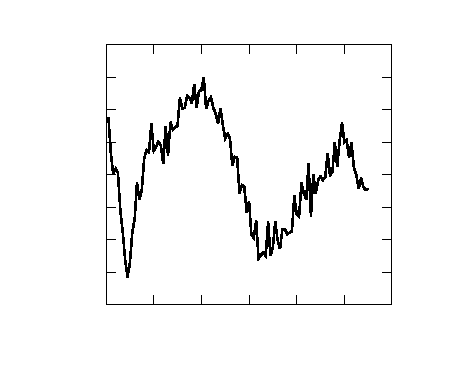
\includegraphics{./figures/parts/02/chapters/01/sections/05/pose_navfn_corridor}}%
    \gplfronttext
  \end{picture}%
\endgroup

     \vspace{0.75cm}
     \caption{\small CORRIDOR}
   \end{subfigure}
   \begin{subfigure}{0.49\linewidth} \centering
     % GNUPLOT: LaTeX picture with Postscript
\begingroup
  \makeatletter
  \providecommand\color[2][]{%
    \GenericError{(gnuplot) \space\space\space\@spaces}{%
      Package color not loaded in conjunction with
      terminal option `colourtext'%
    }{See the gnuplot documentation for explanation.%
    }{Either use 'blacktext' in gnuplot or load the package
      color.sty in LaTeX.}%
    \renewcommand\color[2][]{}%
  }%
  \providecommand\includegraphics[2][]{%
    \GenericError{(gnuplot) \space\space\space\@spaces}{%
      Package graphicx or graphics not loaded%
    }{See the gnuplot documentation for explanation.%
    }{The gnuplot epslatex terminal needs graphicx.sty or graphics.sty.}%
    \renewcommand\includegraphics[2][]{}%
  }%
  \providecommand\rotatebox[2]{#2}%
  \@ifundefined{ifGPcolor}{%
    \newif\ifGPcolor
    \GPcolorfalse
  }{}%
  \@ifundefined{ifGPblacktext}{%
    \newif\ifGPblacktext
    \GPblacktexttrue
  }{}%
  % define a \g@addto@macro without @ in the name:
  \let\gplgaddtomacro\g@addto@macro
  % define empty templates for all commands taking text:
  \gdef\gplfronttext{}%
  \gdef\gplfronttext{}%
  \makeatother
  \ifGPblacktext
    % no textcolor at all
    \def\colorrgb#1{}%
    \def\colorgray#1{}%
  \else
    % gray or color?
    \ifGPcolor
      \def\colorrgb#1{\color[rgb]{#1}}%
      \def\colorgray#1{\color[gray]{#1}}%
      \expandafter\def\csname LTw\endcsname{\color{white}}%
      \expandafter\def\csname LTb\endcsname{\color{black}}%
      \expandafter\def\csname LTa\endcsname{\color{black}}%
      \expandafter\def\csname LT0\endcsname{\color[rgb]{1,0,0}}%
      \expandafter\def\csname LT1\endcsname{\color[rgb]{0,1,0}}%
      \expandafter\def\csname LT2\endcsname{\color[rgb]{0,0,1}}%
      \expandafter\def\csname LT3\endcsname{\color[rgb]{1,0,1}}%
      \expandafter\def\csname LT4\endcsname{\color[rgb]{0,1,1}}%
      \expandafter\def\csname LT5\endcsname{\color[rgb]{1,1,0}}%
      \expandafter\def\csname LT6\endcsname{\color[rgb]{0,0,0}}%
      \expandafter\def\csname LT7\endcsname{\color[rgb]{1,0.3,0}}%
      \expandafter\def\csname LT8\endcsname{\color[rgb]{0.5,0.5,0.5}}%
    \else
      % gray
      \def\colorrgb#1{\color{black}}%
      \def\colorgray#1{\color[gray]{#1}}%
      \expandafter\def\csname LTw\endcsname{\color{white}}%
      \expandafter\def\csname LTb\endcsname{\color{black}}%
      \expandafter\def\csname LTa\endcsname{\color{black}}%
      \expandafter\def\csname LT0\endcsname{\color{black}}%
      \expandafter\def\csname LT1\endcsname{\color{black}}%
      \expandafter\def\csname LT2\endcsname{\color{black}}%
      \expandafter\def\csname LT3\endcsname{\color{black}}%
      \expandafter\def\csname LT4\endcsname{\color{black}}%
      \expandafter\def\csname LT5\endcsname{\color{black}}%
      \expandafter\def\csname LT6\endcsname{\color{black}}%
      \expandafter\def\csname LT7\endcsname{\color{black}}%
      \expandafter\def\csname LT8\endcsname{\color{black}}%
    \fi
  \fi
  \setlength{\unitlength}{0.0500bp}%
  \begin{picture}(4000.00,3200.00)%
    \gplgaddtomacro\gplfronttext{%
      \colorrgb{0.00,0.00,0.00}%
      \put(726,440){\makebox(0,0)[r]{\strut{}$0.0$}}%
      \colorrgb{0.00,0.00,0.00}%
      \put(726,796){\makebox(0,0)[r]{\strut{}$0.05$}}%
      \colorrgb{0.00,0.00,0.00}%
      \put(726,1153){\makebox(0,0)[r]{\strut{}$0.10$}}%
      \colorrgb{0.00,0.00,0.00}%
      \put(726,1509){\makebox(0,0)[r]{\strut{}$0.15$}}%
      \colorrgb{0.00,0.00,0.00}%
      \put(726,1866){\makebox(0,0)[r]{\strut{}$0.20$}}%
      \colorrgb{0.00,0.00,0.00}%
      \put(726,2222){\makebox(0,0)[r]{\strut{}$0.25$}}%
      \colorrgb{0.00,0.00,0.00}%
      \put(726,2579){\makebox(0,0)[r]{\strut{}$0.30$}}%
      \colorrgb{0.00,0.00,0.00}%
      \put(726,2935){\makebox(0,0)[r]{\strut{}$0.35$}}%
      \colorrgb{0.00,0.00,0.00}%
      \put(858,220){\makebox(0,0){\strut{}$0$}}%
      \colorrgb{0.00,0.00,0.00}%
      \put(1544,220){\makebox(0,0){\strut{}$50$}}%
      \colorrgb{0.00,0.00,0.00}%
      \put(2231,220){\makebox(0,0){\strut{}$100$}}%
      \colorrgb{0.00,0.00,0.00}%
      \put(2917,220){\makebox(0,0){\strut{}$150$}}%
      \colorrgb{0.00,0.00,0.00}%
      \put(3603,220){\makebox(0,0){\strut{}$200$}}%
    }%
    \gplgaddtomacro\gplfronttext{%
    }%
    \put(0,0){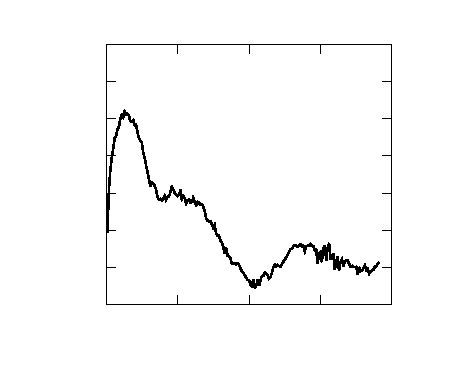
\includegraphics{./figures/parts/02/chapters/01/sections/05/pose_globalplanner_willowgarage}}%
    \gplfronttext
  \end{picture}%
\endgroup

     \vspace{0.75cm}
     \caption{\small WILLOWGARAGE}
   \end{subfigure}
\caption{\small Μέσος όρος σφαλμάτων εκτίμησης στάσης κατά τη διάρκεια του
         χρόνου σε δέκα πειράματα αυτόνομους πλοήγησης με τη χρήση φίλτρου
         σωματιδίων}
\label{fig:02_01_05}
\end{figure}
